% ECIR 2027 full-paper submission draft, with completed v10 diagnostics.
% Springer LNCS; maximum 12 content pages, references excluded.
% Double blind: keep authors, acknowledgments, artifact metadata, and paths anonymous.
% Numerical sources: versioned reports under paper/generated/.
% Rerun the submission audit and inspect the compiled PDF after editing.

\documentclass[runningheads]{llncs}

\usepackage[T1]{fontenc}
\usepackage[utf8]{inputenc}
\usepackage{amsmath}
\usepackage{amssymb}
\usepackage{booktabs}
\usepackage{microtype}
\usepackage{url}
\usepackage{pgfplots}
\pgfplotsset{compat=1.18}
\usepackage[hidelinks]{hyperref}

\newcommand{\method}{\textsc{ACE}}
\newcommand{\norm}[1]{\left\lVert #1 \right\rVert_2}

% Enable only for the non-anonymous version; keep false during review.
\newif\ifincludeacknowledgements
\includeacknowledgementsfalse

\begin{document}

\title{Learning the Center or Exploring Its Neighborhood?\\
A Controlled Study of Multi-Probe Session Retrieval}
\titlerunning{Learning the Center or Exploring Its Neighborhood?}

\author{Anonymous Authors}
\authorrunning{Anonymous Authors}
\institute{Anonymous Institution}

\maketitle

\begin{abstract}
Multi-query retrieval can improve a representation and increase its scoring
budget simultaneously, making the source of a gain difficult to establish.
We study this attribution problem by separating query-center estimation,
local multi-probe expansion, and query-dependent radius adaptation.
Adaptive Centroid Expansion (\method) provides a controlled test across four
item-retrieval datasets, with content, session-neighbor, transition, and
sequential controls under one exact full-catalog evaluator.
Learning the center improves on metadata weighting on two datasets. However,
with selected centers frozen, probe directions paired, and validation averaged
over ten inference seeds, neither fixed-radius expansion over a single center
query nor radius adaptation over a per-center fixed radius shows a clear
incremental gain. This persists with a twelve-value radius grid and two
adaptive parameterizations. Increasing the number of probes from one to twenty
changes TalkPlay ranking performance little; high probe overlap recurs on
validation and test while scoring cost increases.
These findings concern local isotropic probes, max-score aggregation, and the
evaluated uniformly sampled-negative objective. They motivate controlling query
representation, probe directions, and selection and scoring budgets when
attributing gains to adaptive exploration.
\keywords{Session-based recommendation \and Dense retrieval \and Multi-vector
retrieval \and Query expansion \and Full-catalog evaluation}
\end{abstract}

\section{Introduction}
\label{sec:introduction}

Session-based retrieval infers a useful item from a short interaction history.
In embedding-based retrieval, a normalized context mean provides one query;
weighting or attention can improve its location, while additional probes search
its neighborhood. Comparing an adaptive multi-probe retriever only with an
unweighted mean conflates center estimation, probe multiplicity, and radius
adaptation. An overall gain cannot identify which intervention helped.

We use Adaptive Centroid Expansion (\method) to study the decomposition.
It learns a bounded correction to the context centroid and a radius-control
parameter for local tangent-space probes. Catalog embeddings stay frozen;
one scorer supports weighted or learned centers with no, fixed, or adaptive
expansion. To isolate the radius mechanism, we freeze selected centers, pair
probe directions, and match validation inference seeds and selection unit.

We also compare popularity, last-item similarity, transitions, recency-weighted
vector session-kNN (V-SKNN), and content-SASRec under identical prediction
events, exclusions, and complete catalogs. These compare retrieval
configurations, not disjoint information sources: both learned centroids and
content-SASRec use fixed content vectors and interaction supervision. Held-out
prediction events are excluded from training, selection uses validation, and
training and inference randomness are distinguished.

We ask: \textbf{RQ1}, when does learning the center improve content retrieval?
\textbf{RQ2a}, with that center fixed, does local expansion help?
\textbf{RQ2b}, does adaptation improve on a validation-selected fixed radius?
\textbf{RQ3}, how do these methods compare with session-neighbor, transition,
and sequential retrieval?

We contribute a mechanism-focused account of query quality versus multiplicity:
\begin{itemize}
  \item a controlled evaluation design separating query-center estimation
  from local multi-probe exploration;
  \item a full-catalog study across four heterogeneous datasets, with content,
  session-neighbor, transition, and sequential retrieval controls; and
  \item evidence that centering can help, while isotropic probes and adaptive
  radius offer little demonstrated incremental value with the selected center
  fixed, together with their uncertainty and scoring cost.
\end{itemize}
Our empirical conclusions are conditional on isotropic probes, max aggregation,
and the sampled-negative objective; they do not establish results for other
multi-vector systems.

\section{Related Work}
\label{sec:related}

\paragraph{Session and sequential recommendation.}
GRU4Rec, NARM, SR-GNN, SASRec, and BERT4Rec model short-term behavior with
recurrent, attentive, graph, or Transformer architectures
\cite{hidasi2016session,li2017narm,wu2019srgnn,kang2018sasrec,sun2019bert4rec}.
Matched studies nevertheless show that nearest-neighbor and rule-based session
methods remain unusually strong and that protocol and seed choices can change
conclusions \cite{ludewig2018evaluation,shehzad2024comparison}. We therefore
compare against both whole-session neighbors and a causal content-SASRec model;
a first-order transition counter alone would not represent either family.

\paragraph{Multiple representations and interests.}
MIND and ComiRec learn several user vectors for retrieval
\cite{li2019mind,cen2020comirec}; kNN-Embed queries a mixture of locally smoothed
interests \cite{elkishky2022knnembed}. ColBERT preserves multiple query and
document vectors \cite{khattab2020colbert}. Representation learning and vector
multiplicity can therefore change together. Token pooling and constant-space
encodings explicitly study document-side vector budgets
\cite{clavie2024pooling,macavaney2025constant}. We examine a narrower query-side
question: does local expansion help when the center and sampled directions
are held fixed? Our isotropic probes are not learned semantic interests, so
their results do not establish the behavior of these architectures.

\paragraph{Feedback and dense query expansion.}
Classical feedback moves or expands a query using associated evidence
\cite{rocchio1971feedback,lavrenko2001relevance}. Dense PRF extends this to
continuous representations \cite{yu2021denseprf,li2022denseprf}, including
late-interaction feedback \cite{wang2021multirepprf}. Here the evidence is the
observed session, not first-pass retrieved documents. Weighting changes its
center; extra vectors expand the query. Our contribution tests whether a small
separately optimized advantage persists with shared centers and directions,
without claiming that prior work uniformly lacks appropriate controls.

\paragraph{Evaluation.}
Sampled-negative ranking can alter absolute metrics and method orderings
\cite{krichene2020sampled}. We use exact full-catalog ranks and distinguish
prediction events, user/session clusters, training seeds, and inference seeds.
This matters most for small incremental effects: an interval that conditions on
fitted models does not establish stability across retraining.

\section{Task and Method}
\label{sec:method}

\subsection{Full-Catalog Session Retrieval}

Let $\mathcal{V}$ be a catalog with fixed unit vectors
$x_j\in\mathbb{R}^{d}$. A prediction event contains an ordered observed history
$H=(i_1,\ldots,i_t)$ and one target $y\notin H$. The model uses the most recent
$\min(t,10)$ items, denoted $A$, but masks the complete history $H$ before
ranking. It assigns a score to every eligible item in
$\mathcal{V}\setminus H$. The task is held-out-item session retrieval: the
target is excluded from the observed history but may have appeared in
training. The evaluated models consume no dialogue utterances.

The reference query is the normalized context mean
\begin{equation}
 q=\operatorname{norm}\!\left(\sum_{i\in A}x_i\right),\qquad
 \operatorname{norm}(v)=\frac{v}{\max(\norm{v},\epsilon)}.
 \label{eq:mean}
\end{equation}
A metadata-weighted center uses $\sum_i w_i x_i$, where $w_i$ is the normalized
BM25 score of context item $i$ against concatenated context metadata. BM25 uses
$k_1=1.5$, $b=.75$, full-catalog document frequencies, lowercased \verb|\w+|
tokens, repeated query terms, and no stemming or stop-word removal; zero total
score falls back to uniform weights. The artifact specifies the exact formula.
Only static metadata and observed context enter this computation, not dialogue
or target text. ``Weighted PRF'' survives only as an artifact filename.

\subsection{Bounded Learned Center}

The learned center uses $q$ as a single cross-attention query and the context
vectors $X_A$ as keys and values. With multi-head attention (MHA), a two-layer
GELU feed-forward network (FFN), and layer normalization (LN),
\begin{align}
 r&=\operatorname{MHA}(q,X_A,X_A),
 &h&=\operatorname{LN}_1(q+r),\\
 u&=\operatorname{norm}\!\left(\operatorname{LN}_2(r+\operatorname{FFN}(h))\right),
 &\mu&=\operatorname{norm}(q+g u),
 \label{eq:center}
\end{align}
where $g=0.2\sigma(a)$ starts at $a=-2$. Four attention heads, FFN width $4d$,
and dropout .1 are used. The evaluated second residual is
$r+\operatorname{FFN}(h)$, not the conventional $h+\operatorname{FFN}(h)$;
$q$ still enters through $h$ and the outer gated sum. For unit $q,u$,
$\angle(q,\mu)\leq\arcsin(g)<11.54^\circ$, so the model refines the content
center locally. Content-SASRec has no corresponding angular constraint.

\subsection{Fixed and Adaptive Neighborhoods}

For adaptive expansion, a two-layer GELU head predicts
\begin{equation}
 \kappa=\operatorname{clip}\!\left(500\sigma(\operatorname{MLP}(q+gu))+1,
 10,500\right).
 \label{eq:kappa}
\end{equation}
The clamp has zero derivative outside its interval. We also test the smooth
mapping $\kappa=10+490\sigma(\operatorname{MLP}(q+gu))$ on the same frozen
centers (Section~\ref{sec:frozen-results}).
Separately trained fixed variants select $\kappa\in\{10,50,100,500\}$ on
validation data; the frozen-center analysis uses the finer grid below.
For each direction $s$, Gaussian noise is projected into the tangent
space at $\mu$ and normalized:
\begin{align}
 t_s&=\operatorname{norm}\!\left(
 \epsilon_s-(\epsilon_s^\top\mu)\mu\right),\\
 z_s&=\operatorname{norm}\!\left(
 \mu+\frac{t_s}{\sqrt{\kappa+10^{-6}}}\right),
 \qquad \epsilon_s\sim\mathcal{N}(0,I).
 \label{eq:probes}
\end{align}
An item receives its best probe score,
$\operatorname{score}(j\mid H)=\max_{s\leq S}z_s^\top x_j$; without expansion,
the score is $\mu^\top x_j$. Because $t_s\perp\mu$ and both are unit vectors,
\begin{equation}
 \angle(\mu,z_s)=\arctan\!\left((\kappa+10^{-6})^{-1/2}\right)
 \simeq \arctan(\kappa^{-1/2}).
 \label{eq:angle}
\end{equation}
Thus $\kappa$ controls a deterministic polar radius and randomness controls only
the tangent direction. This is fixed-radius tangent expansion, not exact
von Mises--Fisher sampling or calibrated uncertainty
\cite{mardia2000directional}.
Writing $\alpha=(\kappa+10^{-6})^{-1/2}$, the unit-vector geometry also gives
\begin{equation}
 \operatorname{score}(j\mid H)=
 \frac{\mu^\top x_j+\alpha\max_{s\leq S}t_s^\top x_j}
 {\sqrt{1+\alpha^2}}.
 \label{eq:score-decomposition}
\end{equation}
The denominator is item-independent. Adaptation rescales random tangent
scores; it does not learn semantic interests. Isotropic directions isolate
radius scaling from learned direction selection, making this a controlled
test of local exploration under max aggregation.

Learned variants optimize cross-entropy over the target and 64 negatives drawn
from training items, with temperature 0.07. The complete observed history and
target are excluded from negatives. Validation and test remain exhaustive.
Separately trained configurations combine expansion, center optimization, and
training variation. The frozen-center analysis isolates radius changes by
fitting only a radius head on each selected learned-center checkpoint.

\section{Experimental Design}
\label{sec:experiments}

\subsection{Data and Splits}

\begin{table}[t]
\centering\scriptsize
\setlength{\tabcolsep}{3pt}
\caption{Frozen catalogs and retained prediction events. Last.fm is unordered
artist retrieval, not chronological next-item prediction.}
\label{tab:datasets}
\begin{tabular}{lrrrrl}
\toprule
Dataset & Catalog & Train & Valid. & Test & Item representation\\
\midrule
TalkPlay & 46,579 & 95,746 & 1,520 & 1,000 & CLAP audio, 512d\\
MovieLens-1M & 3,883 & 557,170 & 6,034 & 6,034 & MiniLM text, 384d\\
Last.fm & 17,632 & 87,170 & 1,877 & 1,877 & MiniLM name, 384d\\
Amazon Digital Music & 70,537 & 8,973 & 1,221 & 1,221 & MiniLM text, 384d\\
\bottomrule
\end{tabular}
\end{table}

TalkPlayData \cite{musiccrs2026} supplies frozen CLAP vectors
\cite{elizalde2023clap}. Each JSON conversation defines a session; only
\texttt{music} turns are retained in stored order, with \texttt{content} as
track ID. Dialogue and profiles are unused. Official test sessions stay
separate; 10\% of training sessions form deterministic whole-session
validation. Training events are prefixes. Duplicate training, train--test,
and repeated test sequences are removed.

MovieLens-1M \cite{harper2015movielens} and Amazon Digital Music
\cite{hou2026blair} retain ratings $\geq4$ and users with at least five distinct
positive items. Timestamp-ordered interactions are deduplicated; penultimate
and final items are validation and test targets. Test history includes the
validation item. These per-user holdouts have no global time cutoff; other
users' training events may postdate a test event. HetRec Last.fm
\cite{cantador2011hetrec} lacks chronology: artists receive a deterministic
hash order before final-two holdout, and listening counts are discarded.
It is an unordered set-completion stress test.

The hash-frozen \texttt{sentence-transformers/all-MiniLM-L6-v2} snapshot uses
mean pooling and $\ell_2$ normalization \cite{reimers2019sbert,wang2020minilm}.
Text is title/genres for MovieLens, artist name for Last.fm, and title/store
metadata before ``Format:'' for Amazon. TalkPlay BM25 uses title/artist.
Missing-embedding and repeated-target events are rejected without target
substitution. Catalog metadata are transductive; held-out prediction labels
are excluded from training.

Dataset differences in chronology, support, size, event construction, and
modality prevent causal explanations from cross-dataset rankings.

\subsection{Comparators and Selection}

We evaluate popularity, last-item cosine similarity, and first-order transitions
with popularity backoff. V-SKNN indexes the longest training prefix per group
as a binary vector, retrieves neighbors by cosine similarity to a
recency-weighted context, and sums similarity-weighted recency votes for items.
Validation selects $K\in\{50,100,250,500\}$ and $\lambda\in\{.7,.85,1\}$;
the artifact specifies scoring, backoff, and selections. All prefixes with the
active group identifier are excluded. This conservatively prevents the
training-derived prefix from serving as its own neighbor, but on per-user
datasets also discards legitimate same-user history. It is a conservative
comparator choice, not a necessary leakage restriction or a claim about the
best attainable personalized V-SKNN.

Content-SASRec projects frozen item vectors to 256 dimensions, applies two
four-head causal Transformer layers, and projects the last valid state back to
the catalog space. Validation selects learning rate from
$\{10^{-4},3\!\times\!10^{-4}\}$ and dropout from $\{.1,.2\}$. This tests
a sequential architecture using the same item representations, without matching
the centroid model's capacity or angular constraint.

The six content configurations are uniform, weighted, and learned centers;
weighted and learned centers with fixed radius; and a learned center with
adaptive radius. The three neural configurations train separately. AdamW uses
learning rate $10^{-4}$, weight decay .01, batch size 128, and gradient clipping
at 1 for at most 50 epochs. Validation NDCG@10 selects checkpoints with patience
seven. Content-SASRec and the neural center variants use training seeds
$\{42,123,456,789,2026\}$. Fixed radii use validation averages over inference
seeds $\{3101,\ldots,3110\}$. We fixed $S=5$ in the versioned fit configuration,
outside the selection grid; fit and test manifests record it. Test metrics
never select configurations.

For controlled radius analysis, we freeze each validation-selected learned
center and fit hard-clipped or smoothly bounded heads from its original head
initialization. Epoch selection and stopping average validation NDCG@10 over
all ten inference seeds. We compare no expansion with fixed radii from
$\kappa\in\{10,20,35,50,75,100,150,250,350,400,450,500\}$.
The primary fixed control selects per center; a secondary control selects
globally. Expanded conditions share five directions per event and inference
seed. Test averages five centers and ten inference seeds. Centers, directions,
probe count, and selection unit are matched; search spaces and tuning cost are
not. Head epochs and diagnostics are retained. This post-hoc analysis uses
validation for every choice, but cannot explain the original separately
trained gap.

\subsection{Evaluation and Uncertainty}

Every method ranks the complete catalog after masking the complete observed
history. NDCG@10 is primary because it discounts the single target's position
within the first ten ranks and is the configured validation-selection metric;
Recall@10, Recall@50, and MRR@50 are secondary and retained in the artifact.
Single-target ties are broken by ascending canonical catalog index. One
evaluator is shared across methods, datasets, and seeds.

Stochastic means average training and inference seeds; training SD follows
inference averaging. Standard paired intervals average repetitions per event
then cluster-bootstrap users/sessions 10,000 times, conditioning on fitted
models. Central TalkPlay and frozen-center contrasts also cross-resample five
training seeds, ten inference seeds, and user/session clusters, pairing methods
and preserving the event-average estimand. With only five fitted models, the
crossed analysis provides coarse evidence about retraining variability rather
than a precise estimate of its distribution. Intervals are exploratory and
uncorrected; crossing zero does not establish equivalence. The artifact details
the Cartesian-product
draws and retains the historical ``hierarchical'' filename.

\section{Results}
\label{sec:results}

\begin{table}[t]
\centering\scriptsize
\setlength{\tabcolsep}{2pt}
\caption{Exact full-catalog NDCG@10. Neural cells show mean $\pm$ training-seed
SD after averaging inference seeds; weighted+fixed-radius instead shows
inference-seed SD. These describe different randomness sources and are not
directly comparable across all rows. Deterministic cells have no seed SD. Typesetting does not
encode statistical significance.}
\label{tab:main-results}
\begin{tabular}{lrrrr}
\toprule
Method & TalkPlay & MovieLens & Last.fm & Amazon Digital Music\\
\midrule
Popularity & .00033 & .02046 & .03339 & .00000\\
Last item & .01685 & .02252 & .00463 & .05602\\
Transition & .02108 & .10279 & .03552 & .00491\\
V-SKNN & .04887 & .08565 & .09533 & .00932\\
Content-SASRec & $.01871\!\pm\!.00154$ & $.10048\!\pm\!.00144$ & $.03697\!\pm\!.00133$ & $.00885\!\pm\!.00206$\\
\midrule
Uniform center & .02120 & .01314 & .01451 & .05145\\
Weighted center & .02585 & .01397 & .01351 & .05560\\
Learned center & $.02461\!\pm\!.00042$ & $.01864\!\pm\!.00039$ & $.01742\!\pm\!.00061$ & $.05173\!\pm\!.00031$\\
Weighted+fixed-radius & $.02465\!\pm\!.00054$ & $.01387\!\pm\!.00032$ & $.01386\!\pm\!.00027$ & $.05544\!\pm\!.00032$\\
Learned+fixed-radius & $.02548\!\pm\!.00101$ & $.01871\!\pm\!.00032$ & $.01761\!\pm\!.00048$ & $.05203\!\pm\!.00014$\\
\method{} adaptive & $.02600\!\pm\!.00105$ & $.01872\!\pm\!.00052$ & $.01749\!\pm\!.00070$ & $.05205\!\pm\!.00022$\\
\bottomrule
\end{tabular}
\end{table}

\subsection{Comparison with Established Retrieval Configurations}

Table~\ref{tab:main-results} shows no single method ordering across datasets.
Relative
to adaptive \method{}, V-SKNN gains 0.02287 NDCG@10 on TalkPlay (95\% interval
for \method{} adaptive$-$V-SKNN $[-0.03521,-0.01011]$), 0.06693 on MovieLens
($[-0.07278,-0.06112]$), and 0.07784 on Last.fm
($[-0.08800,-0.06774]$). V-SKNN is best on TalkPlay and Last.fm; first-order
transitions are best on MovieLens, closely followed by content-SASRec. These
rankings compare selected configurations with unequal architecture and tuning
grids, not the best attainable member of each method family. The Last.fm result
concerns unordered user--artist overlap;
its transition and Transformer results are stress tests under an imposed
ordering, not temporal sequence evidence.

On Amazon Digital Music, adaptive \method{} exceeds V-SKNN by
0.04273 ($[0.03229,0.05408]$), while last-item and weighted-center retrieval
remain numerically stronger than \method{} (adaptive$-$Last-item interval
$[-0.01333,0.00532]$). Training-item support qualifies this apparent reversal.

\begin{table}[t]
\centering\scriptsize
\setlength{\tabcolsep}{2pt}
\caption{Training-item support and conditional test NDCG@10. Warm means the
target occurs in a training context or target; cold is its complement.
Catalogs and saved rankings are unchanged. ACE denotes the separately trained
adaptive model. V-SKNN cold NDCG@10 is zero on every dataset.}
\label{tab:target-support}
\begin{tabular}{lrrrrrr}
\toprule
Dataset & Cold valid.\% & Cold test\% & Warm $n$ & Warm ACE & Warm V-SKNN & Cold ACE\\
\midrule
TalkPlay & 25.00 & 46.00 & 540 & .01701 & .09051 & .03656\\
MovieLens & .07 & .08 & 6,029 & .01869 & .08572 & .05719\\
Last.fm & 11.51 & 11.40 & 1,663 & .01975 & .10760 & .00000\\
Amazon Digital Music & 86.16 & 87.06 & 158 & .07880 & .07204 & .04808\\
\bottomrule
\end{tabular}
\end{table}

Table~\ref{tab:target-support} partitions saved rankings by training-item
support, without filtering candidates or retuning. On Amazon, 1,063 of 1,221
test targets are cold. Among the 158 warm targets, ACE and V-SKNN score
.07880 and .07204; last-item and weighted-center retrieval score .09379 and
.09196. Thus the aggregate gap cannot be read as a general advantage of the
content family. On TalkPlay, V-SKNN's advantage persists on warm targets,
whereas ACE retrieves some cold targets. Warm status is global training
occurrence, not guaranteed evidence in a method's neighbors. These post-hoc
subsets are descriptive, not causal or significance tests; MovieLens has only
five cold test events. Training support must accompany cross-family comparisons.

\subsection{Center Estimation and Neighborhood Exploration}

Learning the center is the more repeatable intervention within the content
family. Learned minus weighted center is $+0.00467$ on MovieLens
($[0.00337,0.00603]$) and $+0.00391$ on Last.fm
($[0.00197,0.00602]$), but inconclusive on TalkPlay and Amazon Digital Music.
Metadata weighting is numerically strongest on Amazon Digital Music. No center estimator dominates all
representation--catalog pairs.

Fixed-radius expansion helps the separately trained learned TalkPlay center by $+0.00087$
($[0.00005,0.00177]$ under the model-conditional cluster bootstrap) but harms
the weighted center by $-0.00120$ ($[-0.00239,-0.00020]$). This motivates testing
expansion conditional on a shared center. On MovieLens, Last.fm, and
Amazon Digital Music, neither fixed-radius nor adaptive-radius expansion clearly
improves its separately optimized learned-center comparator.

At $S=5$, adaptive \method{} exceeds the separately trained
learned+fixed-radius configuration on TalkPlay by 0.000526. The
model-conditional cluster interval is $[0.00003,0.00108]$, but the five
training-seed differences are $[0.00031,0.00164,0.00054,0.00076,-0.00062]$.
The crossed-bootstrap interval that also resamples training and inference seeds is
$[-0.00049,0.00162]$. The data do not support the stronger claim that adaptive
radius provides a reliable incremental improvement beyond fixed-radius
exploration. The controlled test below addresses the remaining
center-confounding concern with matched validation inference seeds.

\subsection{Radius Comparison with Frozen Centers}
\label{sec:frozen-results}

\begin{table}[t]
\centering\scriptsize
\setlength{\tabcolsep}{2pt}
\caption{Frozen-center NDCG@10, averaged over five centers and ten paired
inference seeds. Both fixed-radius and adaptive-epoch selection use ten
validation inference seeds. Global fixed selects one radius per dataset;
per-center fixed selects separately for each center. Hard and smooth denote
adaptive heads; paired uncertainty is shown in Fig.~\ref{fig:frozen-radius}.}
\label{tab:frozen-center-radius}
\begin{tabular}{lrrrrr}
\toprule
Dataset & No expansion & Global fixed & Per-center fixed & Hard & Smooth\\
\midrule
TalkPlay & .024609 & .024771 & .024775 & .024778 & .024777\\
MovieLens & .018642 & .018588 & .018600 & .018609 & .018598\\
Last.fm & .017421 & .017334 & .017344 & .017316 & .017327\\
Amazon Digital Music & .051729 & .051780 & .051892 & .051953 & .051871\\
\bottomrule
\end{tabular}
\end{table}

Table~\ref{tab:frozen-center-radius} tests the radius mechanism without changing
the selected center. On TalkPlay, hard adaptation exceeds per-center fixed
radius by only $+.000002$, compared with $+.00053$ between separately trained
configurations. Training and selection also differ between these protocols,
so this change does not identify the cause of the original gap. Every hard-
and smooth-versus-per-center-fixed interval includes zero
(Fig.~\ref{fig:frozen-radius}); the same holds against global fixed radius and
for smooth versus hard adaptation. The largest hard-minus-per-center-fixed
point estimate is $+.000061$ on Amazon Digital Music, with interval
$[-.000131,+.000270]$. These are unresolved small effects, not equivalence tests.

Neither global nor per-center fixed expansion clearly improves on no expansion
on any dataset. Global selection chooses $\kappa=500$ throughout, the smallest
angular radius in the twelve-value grid. Per-center choices are not constant:
they span 450--500 on TalkPlay, 20--500 on MovieLens, 350--500 on Last.fm, and
20--400 on Amazon Digital Music. Thus the finer grid permits different selected
radii without establishing an adaptive advantage. An earlier control matching
both selections to a single validation inference seed likewise found no clear
advantage; its results are retained in the artifact. The primary analysis above
uses ten seeds for both procedures and does not reuse earlier selected heads.

Secondary point estimates show similarly small, mixed effects: per-center
fixed minus no expansion stays below .00057 in absolute Recall@10 and .00012
in MRR@50; either adaptive head minus per-center fixed stays below .00014 and
.00004, respectively, across datasets. These descriptive checks support the
qualitative pattern, but uncertainty tests remain specific to NDCG@10.

\begin{figure}[t]
\centering
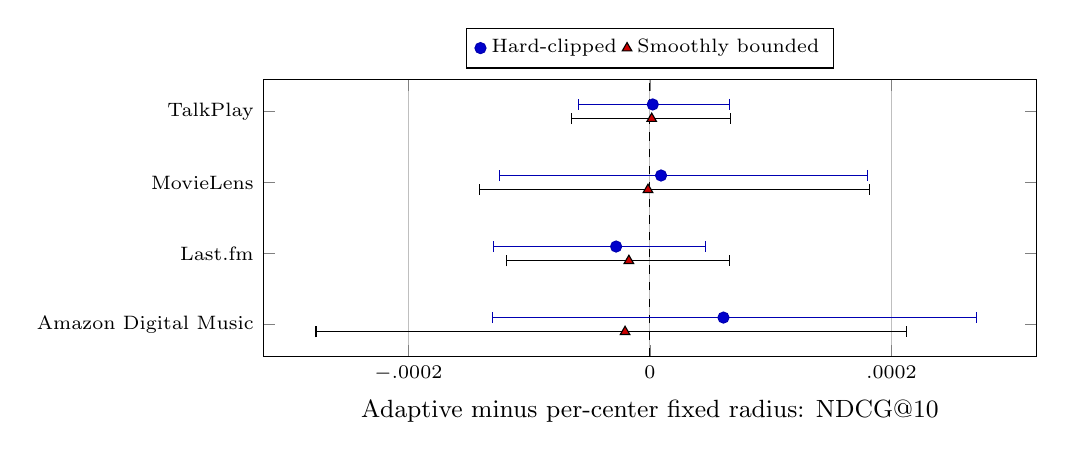
\begin{tikzpicture}
\begin{axis}[width=.94\linewidth,height=5.1cm,
  xmin=-.00032,xmax=.00032,ymin=.55,ymax=4.45,
  ytick={1,2,3,4},yticklabels={Amazon Digital Music,Last.fm,MovieLens,TalkPlay},
  xtick={-.0002,0,.0002},scaled x ticks=false,
  xticklabels={$-.0002$,$0$,$.0002$},
  xlabel={Adaptive minus per-center fixed radius: NDCG@10},
  tick label style={font=\scriptsize},label style={font=\small},
  legend style={font=\scriptsize,at={(.5,1.04)},anchor=south,legend columns=2},
  xmajorgrids=true]
\addplot[black,dashed,forget plot] coordinates {(0,.55)(0,4.45)};
% Source: ecir-radius-v9/*/paired_comparisons.csv, adaptive minus fixed_per_center.
\addplot+[only marks,mark=*,blue!70!black,error bars/.cd,x dir=both,x explicit]
table[x=mean,y=y,x error minus expr=\thisrow{mean}-\thisrow{low},
  x error plus expr=\thisrow{high}-\thisrow{mean}] {
% BEGIN FROZEN HARD
y mean low high
4.1 2.399807445404014e-06 -5.9324125350655416e-05 6.558332525459809e-05
3.1 9.25888684443525e-06 -0.00012424552233205731 0.00017989970015771067
2.1 -2.7938006210971535e-05 -0.0001292591999039918 4.6000504072563705e-05
1.1 6.094464878643146e-05 -0.00013054600135906975 0.0002701800635656003
% END FROZEN HARD
};
\addlegendentry{Hard-clipped}
\addplot+[only marks,mark=triangle*,black,error bars/.cd,x dir=both,x explicit]
table[x=mean,y=y,x error minus expr=\thisrow{mean}-\thisrow{low},
  x error plus expr=\thisrow{high}-\thisrow{mean}] {
% BEGIN FROZEN SMOOTH
y mean low high
3.9 1.5233324286269856e-06 -6.47898260800443e-05 6.689170616000763e-05
2.9 -1.5446629039181657e-06 -0.00014108013096382897 0.00018190981729739402
1.9 -1.7372541394198555e-05 -0.00011836498929095786 6.607135332881271e-05
0.9 -2.054540998768076e-05 -0.00027649221229915523 0.00021214125966288709
% END FROZEN SMOOTH
};
\addlegendentry{Smoothly bounded}
\end{axis}
\end{tikzpicture}
\caption{Frozen-center adaptation versus a fixed radius selected per center.
Points are paired mean effects; bars are descriptive crossed-bootstrap 95\%
intervals over five center seeds, ten inference seeds, and session/user clusters.
Every interval includes zero. Validation inference seeds and selection unit
are matched, not search spaces or tuning cost; these are not equivalence tests.}
\label{fig:frozen-radius}
\end{figure}

\begin{figure}[t]
\centering
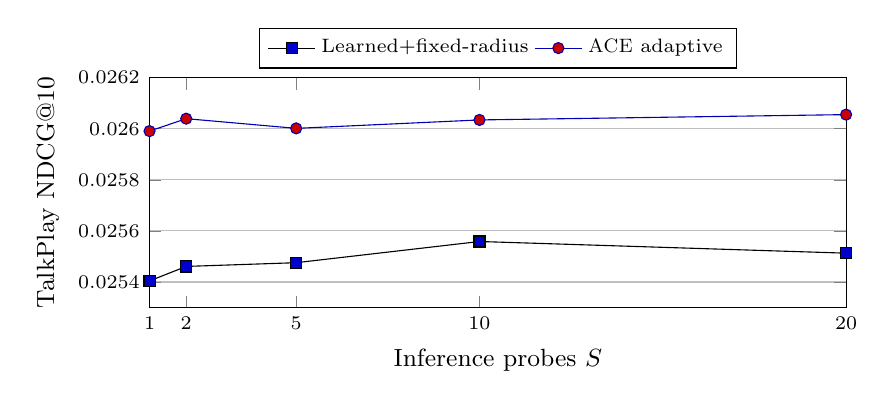
\begin{tikzpicture}
\begin{axis}[width=.86\linewidth,height=4.5cm,
  xmin=1,xmax=20,xtick={1,2,5,10,20},ymin=.0253,ymax=.0262,
  scaled y ticks=false,ytick={.0254,.0256,.0258,.0260,.0262},
  yticklabel style={/pgf/number format/fixed,/pgf/number format/precision=4},
  xlabel={Inference probes $S$},ylabel={TalkPlay NDCG@10},
  tick label style={font=\scriptsize},label style={font=\small},
  legend style={font=\scriptsize,at={(.5,1.04)},anchor=south,legend columns=2},
  ymajorgrids=true]
% Source: ecir-direction-sensitivity-v1/direction_sensitivity.csv.
\addplot+[mark=square*,black] coordinates {
% BEGIN PROBES FIXED
(1,.02540416780904569) (2,.025460887933941467) (5,.0254754910717065)
(10,.025558510112416184) (20,.025512813537570414)
% END PROBES FIXED
};
\addlegendentry{Learned+fixed-radius}
\addplot+[mark=*,blue!70!black] coordinates {
% BEGIN PROBES ADAPTIVE
(1,.025990922137464966) (2,.0260395979231138) (5,.02600158025386467)
(10,.026034643510541227) (20,.02605545890095548)
% END PROBES ADAPTIVE
};
\addlegendentry{\method{} adaptive}
\end{axis}
\end{tikzpicture}
\caption{Inference-only probe-count sensitivity on TalkPlay. Means average
five training and ten paired inference seeds. Both configurations were trained
with $S=5$ and retain their separately optimized checkpoints; this is neither
a retraining comparison nor evidence of significance between curves.
The test sweep does not select $S$.}
\label{fig:direction-sensitivity}
\end{figure}

Figure~\ref{fig:direction-sensitivity} shows little numerical response to probe
count in these frozen checkpoints: across $S=1$--20, learned+fixed-radius varies
by only 0.00015 and adaptive \method{} by 0.00006. Five probes are thus a fixed
reference configuration, not an empirically unique optimum. The persistent gap
between the two curves may reflect their separately trained centers or
different radii; the frozen-center result does not reproduce it as a clear
adaptive-radius effect.

To measure redundancy directly, we inspect each probe's top ten candidates on
all 1,000 TalkPlay test events, averaged over five training and ten inference
seeds. At $S=20$, mean pairwise top-ten Jaccard overlap is .825 for learned+fixed
and .912 for adaptive \method{}; their unions contain only 13.74 and 11.71
distinct items on average. For adaptive \method{}, target inclusion in this
union is .05030, whereas merged Recall@10 is .04736, compared with .04730 at
$S=1$. Union coverage has a larger candidate budget and is not Recall@10.
The overlap is consistent with redundant probes, but neither proves a causal
explanation nor excludes occasional useful new candidates. These diagnostics
use the separately trained models, not the frozen-center heads.

Repeating the diagnostic on all 1,520 validation events gives $S=20$ Jaccard
overlaps .826 and .913, and union sizes 13.75 and 11.70, respectively.
Agreement across splits supports the descriptive redundancy finding. The check
is still post-hoc, uses validation-selected checkpoints, and selects no new
model, radius, or probe count; it is not independent confirmatory evidence.

\subsection{What Does the Adaptive Radius-Control Parameter Learn?}

In the separately trained full model, 99.9\% of TalkPlay validation queries
reach $\kappa=500$, and 100.0\% of Last.fm queries reach $\kappa=10$.
MovieLens and Amazon exhibit radius variation (full diagnostics in the
artifact). The smooth frozen-center head removes clamp-induced zero gradients
but yields no clear gain. This does not identify the cause of the joint
model's boundary states: sigmoid saturation and optimization limitations remain.

\subsection{Randomness and Cost}

The TalkPlay event-cluster interval is positive, while the interval over five
fitted models includes zero; the artifact separates training and inference SD.
On Amazon, single-query versus five-probe adaptive scoring takes .079 versus
.291 ms/query (3.7 times), with median total time .307 versus .531 ms/query
(73\% higher). Fixed and adaptive probes have similar cost; all timing and
sampled-memory values are in the artifact. Synchronized float32 measurements
use batch 128, three warm-ups and ten timed batches on one 16-GB Apple M4
MacBook Air with PyTorch 2.14.0. They do not measure ANN or peak memory.

\section{Discussion}
\label{sec:discussion}

\paragraph{Separating representation and retrieval budget.}
Freezing the center, pairing directions, and comparing one query with
validation-selected fixed and adaptive radii separates center quality from
exploration. Matching inference seeds and selection unit strengthens attribution
without equalizing search spaces. Analogous controls may help semantic
multi-query evaluation, but their empirical value is demonstrated here only
for item retrieval with isotropic local probes.

\paragraph{What the conditional finding contributes.}
Equation~\ref{eq:score-decomposition} identifies adaptation as rescaling
isotropic tangent scores combined by maximum. Neither fixed expansion nor
adaptive scaling shows a clear frozen-center advantage under that scoring rule
and the evaluated sampled-negative objective.
The small separately trained gap therefore does not establish a radius benefit;
other learned directions, objectives, and fusion rules remain open.

\paragraph{Implications for multi-query retrieval evaluation.}
Broad controls matter: on TalkPlay, V-SKNN exceeds adaptive \method{} by 0.02287,
while adaptive \method{} exceeds the uniform center by 0.00480. Target support
must also be reported: Amazon's predominantly cold targets expose a substantial
asymmetry between content scoring and interaction evidence. This motivates
warm/cold reporting alongside unchanged full-catalog results, not a causal
rule linking sparsity to a preferred retrieval family.

\section{Limitations, Ethics, and Reproducibility}
\label{sec:limitations}

\paragraph{Scope and validity.}
The evidence concerns item retrieval, with heterogeneous encoders and split
protocols; it does not establish conversational or document-retrieval behavior.
The separately trained comparison confounds radius and center learning. Freezing
selected centers removes that variation but does not test all centers or joint
smooth-head training. The nonstandard $r+\operatorname{FFN}(h)$ residual lacks
a standard-residual control. Uniformly sampled negatives may provide little
signal about locally confusable items; the radius conclusion is conditional on
this objective. Alternative head initializations and optimization schedules are
untested, and retained checkpoints and gradient diagnostics do not establish
convergence. Clipping and sigmoid saturation can both limit learning.

The refined grid, matched head selection, probe sweep, support partition, and
validation-overlap check are post-hoc analyses of existing splits. They are
not independent confirmation and do not select new configurations from test
results. Grid and epoch search differ in capacity and cost. Warm/cold subsets
are descriptive; their uncertainty and causal role are not established.

\paragraph{Method coverage and systems scope.}
The comparators do not exhaust neural or hybrid models; V-SKNN's same-group
exclusion is conservative. Exact scoring does not establish ANN recall or
production performance. Radius is not calibrated uncertainty. One Apple-MPS
system and ten timed batches limit cost generalization. Five fitted models
give coarse retraining evidence, and accelerator nondeterminism may remain.

\paragraph{Ethics.}
Ranking accuracy does not establish fairness, diversity, or user welfare;
these outcomes are not studied. No demographic attributes are used and no
human participants are recruited.

\paragraph{Reproducibility.}
The anonymous artifact documents exact commands, splits, validation selections,
seed lists, and hash-linked results. Tables and figures use the same versioned
reports. Selection never uses test metrics. Raw licensed data and large
checkpoints are not redistributed. Packaging and PDF anonymity checks are
documented in the artifact rather than treated as scientific contributions.

\section{Conclusion}
\label{sec:conclusion}

Separating center estimation from neighborhood exploration makes attribution
testable. Learned centering improves on metadata weighting on two datasets;
neither fixed expansion nor adaptive radius has a clear frozen-center benefit
under the evaluated objective and max scorer. High probe overlap recurs on
TalkPlay validation and test, while training-item support qualifies cross-family
rankings. The contribution is a controlled evaluation protocol and conditional
evidence for isotropic local probes under max aggregation and the evaluated
sampled-negative objective. Query quality, vector budget, target support, and
retrieval cost should be assessed separately.

\ifincludeacknowledgements
\input{paper/acknowledgements-camera-ready.tex}
\fi

% Flush content floats before references so the auxiliary marker gives a
% conservative, auditable content-page boundary after a clean compilation.
\clearpage
\begin{thebibliography}{27}
\label{page:references-start}

\bibitem{cantador2011hetrec}
Cantador, I., Brusilovsky, P., Kuflik, T.:
Second workshop on information heterogeneity and fusion in recommender systems
(HetRec 2011). In: Proceedings of RecSys (2011)

\bibitem{cen2020comirec}
Cen, Y., Zhang, J., Zou, X., Zhou, C., Yang, H., Tang, J.:
Controllable multi-interest framework for recommendation.
In: KDD, pp. 2942--2951 (2020)

\bibitem{clavie2024pooling}
Clavi\'e, B., Chaffin, A., Adams, G.:
Reducing the footprint of multi-vector retrieval with minimal performance
impact via token pooling. arXiv:2409.14683 (2024)

\bibitem{elizalde2023clap}
Elizalde, B., Deshmukh, S., Al Ismail, M., Wang, H.:
CLAP learning audio concepts from natural language supervision.
In: ICASSP, pp. 1--5 (2023)

\bibitem{elkishky2022knnembed}
El-Kishky, A., Markovich, T., Leung, K., Portman, F., Haghighi, A., Xiao, Y.:
kNN-Embed: Locally smoothed embedding mixtures for multi-interest candidate
retrieval. In: PAKDD (2023)

\bibitem{harper2015movielens}
Harper, F.M., Konstan, J.A.:
The MovieLens datasets: History and context.
ACM TiiS 5(4), 1--19 (2015)

\bibitem{hidasi2016session}
Hidasi, B., Karatzoglou, A., Baltrunas, L., Tikk, D.:
Session-based recommendations with recurrent neural networks.
In: ICLR (2016)

\bibitem{hou2026blair}
Hou, Y., Li, J., Fu, X., He, Z., Yan, A., Chen, X., McAuley, J.:
Bridging language and items for retrieval and recommendation: Benchmarking
LLMs as semantic encoders.
In: ACL, pp. 3251--3265 (2026).
\url{https://doi.org/10.18653/v1/2026.acl-long.147}

\bibitem{kang2018sasrec}
Kang, W.-C., McAuley, J.:
Self-attentive sequential recommendation.
In: ICDM, pp. 197--206 (2018)

\bibitem{khattab2020colbert}
Khattab, O., Zaharia, M.:
ColBERT: Efficient and effective passage search via contextualized late
interaction over BERT. In: SIGIR, pp. 39--48 (2020)

\bibitem{krichene2020sampled}
Krichene, W., Rendle, S.:
On sampled metrics for item recommendation.
In: KDD, pp. 1748--1757 (2020)

\bibitem{lavrenko2001relevance}
Lavrenko, V., Croft, W.B.:
Relevance-based language models. In: SIGIR, pp. 120--127 (2001)

\bibitem{li2017narm}
Li, J., Ren, P., Chen, Z., Ren, Z., Ma, J.:
Neural attentive session-based recommendation.
In: CIKM, pp. 1419--1428 (2017)

\bibitem{li2019mind}
Li, C., Liu, Z., Wu, M., Xu, Y., Huang, P., Zhao, H., Kang, G., Chen, Q.,
Li, W., Lee, D.L.:
Multi-interest network with dynamic routing for recommendation at Tmall.
In: CIKM, pp. 2615--2623 (2019)

\bibitem{li2022denseprf}
Li, H., Zhuang, S., Mourad, A., Ma, X., Lin, J., Zuccon, G.:
Improving query representations for dense retrieval with pseudo relevance
feedback: A reproducibility study. In: ECIR, pp. 599--612 (2022)

\bibitem{ludewig2018evaluation}
Ludewig, M., Jannach, D.:
Evaluation of session-based recommendation algorithms.
UMUAI 28, 331--390 (2018)

\bibitem{macavaney2025constant}
MacAvaney, S., Mallia, A., Tonellotto, N.:
Efficient constant-space multi-vector retrieval. arXiv:2504.01818 (2025)

\bibitem{mardia2000directional}
Mardia, K.V., Jupp, P.E.:
Directional Statistics. Wiley (2000)

\bibitem{musiccrs2026}
Music-CRS Challenge:
Conversational music recommendation challenge and TalkPlayData.
\url{https://recsys.acm.org/recsys26/challenge/} (2026)

\bibitem{reimers2019sbert}
Reimers, N., Gurevych, I.:
Sentence-BERT: Sentence embeddings using Siamese BERT-networks.
In: EMNLP-IJCNLP, pp. 3982--3992 (2019)

\bibitem{rocchio1971feedback}
Rocchio, J.J.:
Relevance feedback in information retrieval.
In: Salton, G. (ed.) The SMART Retrieval System, pp. 313--323.
Prentice-Hall (1971)

\bibitem{shehzad2024comparison}
Shehzad, F., Jannach, D.:
Performance comparison of session-based recommendation algorithms based on
GNNs. In: ECIR, pp. 115--131 (2024)

\bibitem{sun2019bert4rec}
Sun, F., Liu, J., Wu, J., Pei, C., Lin, X., Ou, W., Jiang, P.:
BERT4Rec: Sequential recommendation with bidirectional encoder representations
from Transformer. In: CIKM, pp. 1441--1450 (2019)

\bibitem{wang2021multirepprf}
Wang, X., Macdonald, C., Tonellotto, N., Ounis, I.:
Pseudo-relevance feedback for multiple representation dense retrieval.
In: ICTIR, pp. 297--306 (2021)

\bibitem{wang2020minilm}
Wang, W., Wei, F., Dong, L., Bao, H., Yang, N., Zhou, M.:
MiniLM: Deep self-attention distillation for task-agnostic compression of
pre-trained Transformers. In: NeurIPS 33 (2020)

\bibitem{wu2019srgnn}
Wu, S., Tang, Y., Zhu, Y., Wang, L., Xie, X., Tan, T.:
Session-based recommendation with graph neural networks.
In: AAAI 33, pp. 346--353 (2019)

\bibitem{yu2021denseprf}
Yu, H., Xiong, C., Callan, J.:
Improving query representations for dense retrieval with pseudo relevance
feedback. In: CIKM, pp. 2805--2809 (2021)

\end{thebibliography}

\end{document}
